%!TEX root = Manuscript.tex

\chapter{Precise matching}
\label{chap:intro}
\minitoc

\section{Introduction}
\subsection{Motivation}
\subsection{Contribution}
check SIFT scale and rotation\\
\textit{one-to-one tiling scheme}\\
3D ransac?

\section{Methodology}

\begin{figure*}[htbp]
	\begin{center}
		\subfigure[Workflow]{
			\begin{minipage}[t]{1\linewidth}
				\centering
				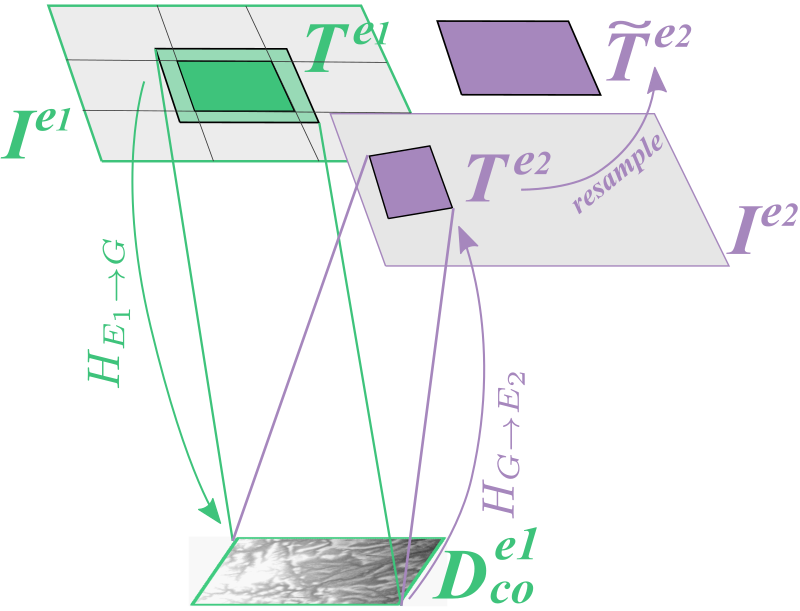
\includegraphics[width=1\columnwidth]{images/Chapitre4/patchmatching.png}
			\end{minipage}%
		}
			\subfigure[Example of an image pair]{
		\begin{minipage}[t]{1\linewidth}
			\centering
			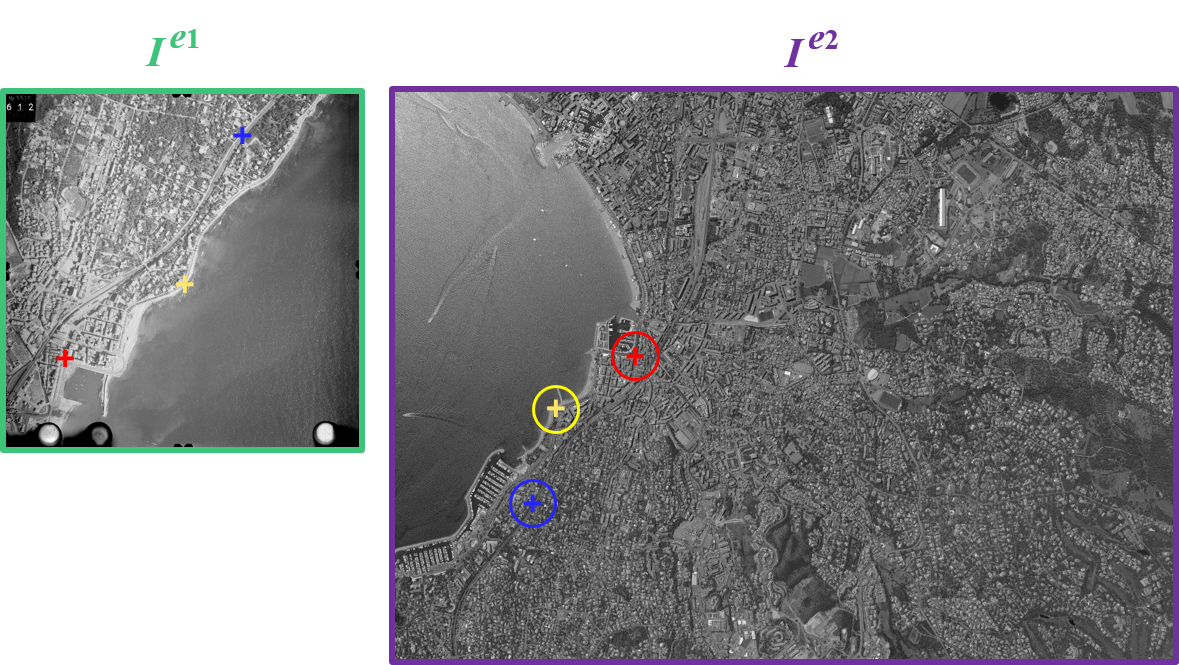
\includegraphics[width=1\columnwidth,trim=0 0 0 50,clip]{images/Chapitre4/guidedexample.png}
		\end{minipage}%
	}
		\subfigure[Example of patch pairs]{
			\begin{minipage}[t]{1\linewidth}
				\centering
				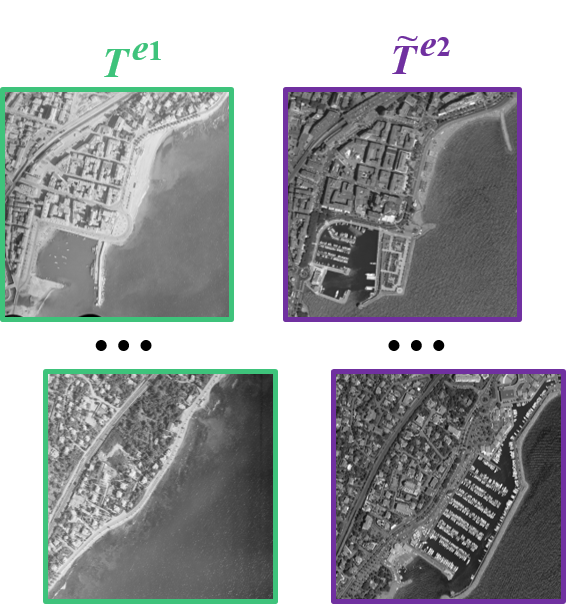
\includegraphics[width=0.5\columnwidth]{images/Chapitre4/patchexample.png}
			\end{minipage}%
		}
		\caption{(a) Workflow of patch matching. (b) Demonstration of an image pair example, the master image ($I^{e_1}$) and secondary image ($I^{e_2}$) are taken at Fr{\'e}jus in 1954 and 2014 individually. (c) Patch pairs resulted from (b).}
		\label{WorkflowPatch}
	\end{center}
\end{figure*}

\begin{figure*}[htbp]
	\begin{center}
		\subfigure[Workflow]{
			\begin{minipage}[t]{1\linewidth}
				\centering
				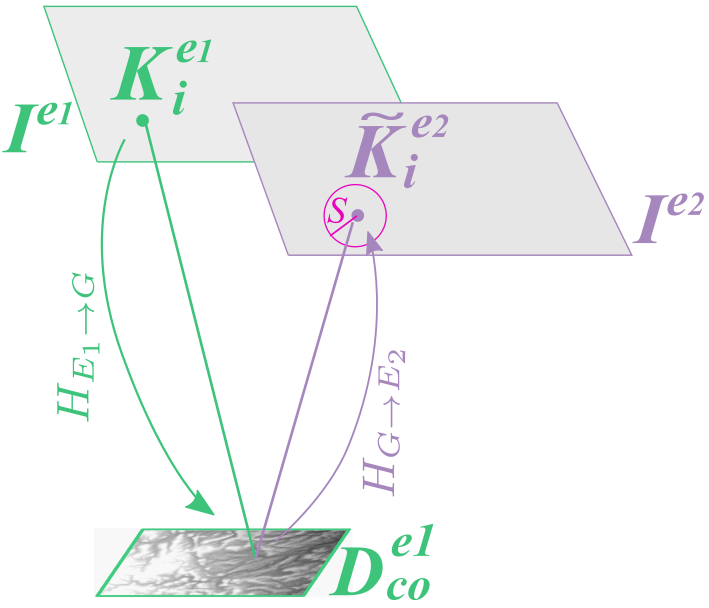
\includegraphics[width=1\columnwidth]{images/Chapitre4/guidedmatching.png}
			\end{minipage}%
		}
		\subfigure[Example of keypoint demonstration]{
			\begin{minipage}[t]{1\linewidth}
				\centering
				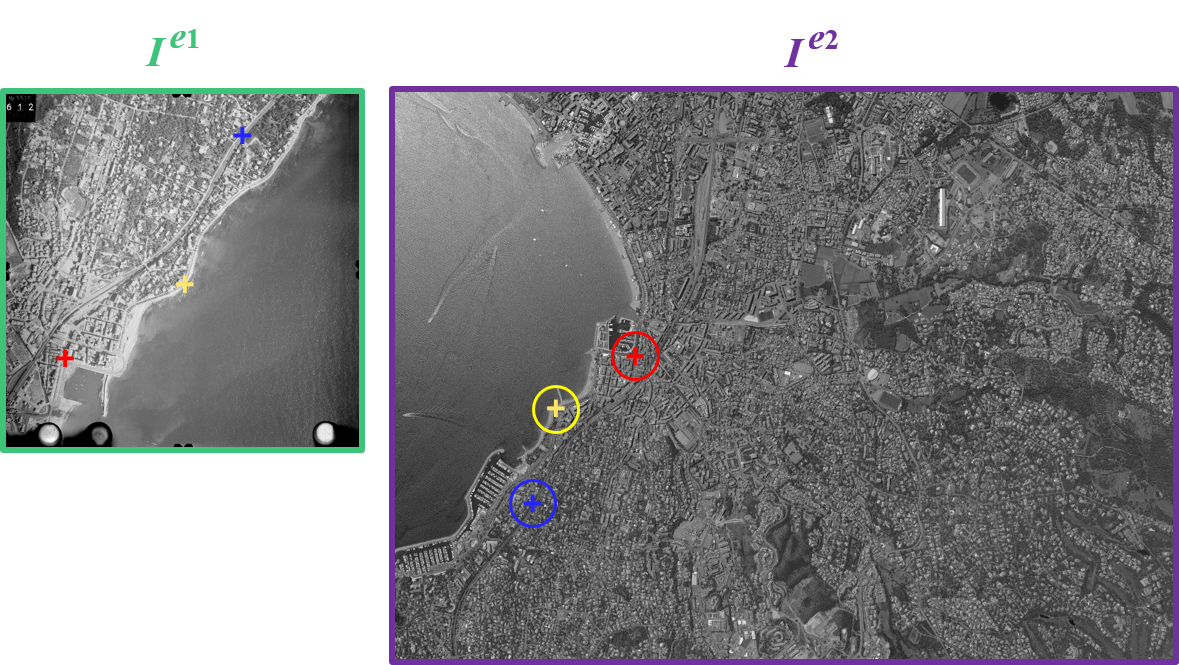
\includegraphics[width=1\columnwidth]{images/Chapitre4/guidedexample.png}
			\end{minipage}%
		}
		\caption{(a) Workflow of guided matching. (b) Demonstration of keypoint prediction accompanied with search space on an image pair example, the master image ($I^{e_1}$) and secondary image ($I^{e_2}$) are taken at Fr{\'e}jus in 1954 and 2014 individually.}
		\label{WorkflowPatch}
	\end{center}
\end{figure*}



\section{Experiments}

\section{Conclusion}

\section{Discussion}
